%%%%%%%%%%%%%%%%%%%%%%%%%%%%%%%%%%%%%%%%%
% Stylish Article
% LaTeX Template
% Version 2.1 (1/10/15)
%
% This template has been downloaded from:
% http://www.LaTeXTemplates.com
%
% Original author:
% Mathias Legrand (legrand.mathias@gmail.com) 
% With extensive modifications by:
% Vel (vel@latextemplates.com)
%
% License:
% CC BY-NC-SA 3.0 (http://creativecommons.org/licenses/by-nc-sa/3.0/)
%
%%%%%%%%%%%%%%%%%%%%%%%%%%%%%%%%%%%%%%%%%

%----------------------------------------------------------------------------------------
%	PACKAGES AND OTHER DOCUMENT CONFIGURATIONS
%----------------------------------------------------------------------------------------

\documentclass[fleqn,10pt]{SelfArx} % Document font size and equations flushed left

\usepackage[english]{babel} % Specify a different language here - english by default

\usepackage{lipsum} % Required to insert dummy text. To be removed otherwise
 
\usepackage{graphicx}
\graphicspath{ {./img/} } %setting images folder
%----------------------------------------------------------------------------------------
%	COLUMNS
%----------------------------------------------------------------------------------------

\setlength{\columnsep}{0.55cm} % Distance between the two columns of text
\setlength{\fboxrule}{0.75pt} % Width of the border around the abstract

%----------------------------------------------------------------------------------------
%	COLORS
%----------------------------------------------------------------------------------------

\definecolor{color1}{RGB}{0,0,90} % Color of the article title and sections
\definecolor{color2}{RGB}{0,20,20} % Color of the boxes behind the abstract and headings

%----------------------------------------------------------------------------------------
%	HYPERLINKS
%----------------------------------------------------------------------------------------

\usepackage{hyperref} % Required for hyperlinks
\hypersetup{hidelinks,colorlinks,breaklinks=true,urlcolor=color2,citecolor=color1,linkcolor=color1,bookmarksopen=false,pdftitle={Title},pdfauthor={Author}}


\usepackage{listings}
\usepackage{color}

\definecolor{dkgreen}{rgb}{0,0.6,0}
\definecolor{gray}{rgb}{0.5,0.5,0.5}
\definecolor{mauve}{rgb}{0.58,0,0.82}

\lstset{frame=tb,
	language=Python,
	aboveskip=3mm,
	belowskip=3mm,
	showstringspaces=false,
	columns=flexible,
	basicstyle={\small\ttfamily},
	numbers=none,
	numberstyle=\tiny\color{gray},
	keywordstyle=\color{blue},
	commentstyle=\color{dkgreen},
	stringstyle=\color{mauve},
	breaklines=true,
	breakatwhitespace=true,
	tabsize=3
}

%----------------------------------------------------------------------------------------
%	ARTICLE INFORMATION
%----------------------------------------------------------------------------------------

\JournalInfo{Università degli Studi di Milano Bicocca} % Journal information
\Archive{ML Project} % Additional notes (e.g. copyright, DOI, review/research article)


\PaperTitle{Machine Learning - Project (Dare Nome piu decente)} % Article title

\Authors{Kasela Pranav\textsuperscript{1}, Pagani Miriam Beatrice\textsuperscript{2}, Saviano Marco\textsuperscript{3}, Zaccaria Antonella\textsuperscript{4}}

\affiliation{\textsuperscript{1}\textit{Matricola: 846965, Department of Informatics, University of Bicocca}} 
\affiliation{\textsuperscript{2}\textit{Matricola: 794274, Department of Informatics, University of Bicocca}}
 \affiliation{\textsuperscript{3}\textit{Matricola: 793516, Department of Informatics, University of Bicocca}}
\affiliation{\textsuperscript{4}\textit{Matricola: 848647, Department of Informatics, University of Bicocca}}

\Keywords{Keyword1 --- Keyword2 --- Keyword3} % Keywords - if you don't want any simply remove all the text between the curly brackets
\newcommand{\keywordname}{Keywords} % Defines the keywords heading name

%----------------------------------------------------------------------------------------
%	ABSTRACT
%----------------------------------------------------------------------------------------

\Abstract{Credit card default happens when you've become severely delinquent on your credit card payment.
	
	It's a serious credit card status that not only affects your standing with that credit card issuer, but also your credit standing in general and your ability to get approved for credit cards, loans, and other credit-based services.
	
	When you accept a credit card, you agree to certain terms, e.g. you agree to make your minimum payment by the due date listed on your credit card statement.
	
	If you miss the minimum credit card payment six months in a row, your credit card will be in default; your credit card issuer will likely close your account and report the default to the credit bureaus.
	
	By the time your credit card defaults, you've likely accumulated hundreds of dollars in fees and interest charges. 
	
	
	Unfortunately, your options for clearing up the credit card default may be limited because of the number of payments you've missed on your account. 
	
	For this reason, assuming truthful the given data, we show the procedure used to create prevision algorithm aiming to foresee the default payment's client.
}

%----------------------------------------------------------------------------------------

\begin{document}
	
	\flushbottom % Makes all text pages the same height
	
	\maketitle % Print the title and abstract box
	
	\tableofcontents % Print the contents section
	
	
	%----------------------------------------------------------------------------------------
	%	ARTICLE CONTENTS
	%----------------------------------------------------------------------------------------
	
	\section*{Introduction\cite{DataSet}} % The \section*{} command stops section numbering
	
	\addcontentsline{toc}{section}{Introduction} % Adds this section to the table of contents
	This dataset is available on Kaggle under the name \textit{Default of Credit Card Clients Dataset} and it  contains information on default payments, demographic factors, credit data, history of payment and bill statements of 30,000 credit card clients in Taiwan from April 2005 to September 2005.
	
	The 25 attributes and their characteristics are:
	\begin{itemize}[noitemsep]
		\item ID: ID of each client
		\item LIMIT\_BAL: Amount of given credit in NT dollars
		\item SEX: Gender (1=male, 2=female)
		\item EDUCATION: (1=graduate school, 2=university, 3=high school, 4=others, 0,5,6=unknown)
		\item MARRIAGE: Marital status (1=married, 2=single, 3=others, 0=others)
		\item AGE: Age in years
		\item PAY\_0: Repayment status in September 2005 (-2=no consumption, 0=use of revolving credit, -1=pay duly, 1=payment delay for one month, 2=payment delay for two months, ... 8=payment delay for eight months, 9=payment delay for nine months and above)
		\item PAY\_2: Repayment status in August, 2005 (scale same as above)
		\item PAY\_3: Repayment status in July, 2005 (scale same as above)
		\item PAY\_4: Repayment status in June, 2005 (scale same as above)
		\item PAY\_5: Repayment status in May, 2005 (scale same as above)
		\item PAY\_6: Repayment status in April, 2005 (scale same as above)
		\item BILL\_AMT1: Amount of bill statement in September 2005 respectively (NT dollar)
		\item BILL\_AMT2: Amount of bill statement in August, 2005 (NT dollar)
		\item BILL\_AMT3: Amount of bill statement in July, 2005 (NT dollar)
		\item BILL\_AMT4: Amount of bill statement in June, 2005 (NT dollar)
		\item BILL\_AMT5: Amount of bill statement in May, 2005 (NT dollar)
		\item BILL\_AMT6: Amount of bill statement in April, 2005 (NT dollar)
		\item PAY\_AMT1: Amount of previous payment in September 2005 respectively (NT dollar)
		\item PAY\_AMT2: Amount of previous payment in August, 2005 (NT dollar)
		\item PAY\_AMT3: Amount of previous payment in July, 2005 (NT dollar)
		\item PAY\_AMT4: Amount of previous payment in June, 2005 (NT dollar)
		\item PAY\_AMT5: Amount of previous payment in May, 2005 (NT dollar)
		\item PAY\_AMT6: Amount of previous payment in April, 2005 (NT dollar)
		\item default.payment.next.month: Default payment (1=yes, 0=no)
	\end{itemize}
	
	%------------------------------------------------
	
	\textbf{Goal:}\newline
	Looking at the problem we see a potential use in predicting month by month, the default of the clients.
	
	\section{Preprocessing}
	Before proceeding with Feature Engineering and the  implementation of Machine Learning, we analyze the dataset with Descriptive Statistics in order to understand more the composition and tendencies of our data.
	
	We notice that in the attribute \textit{EDUCATION} the values 0,5 and 6 are unknown while the value 4 is other, so we decide to categorize 0,5 and 6 as other too.
	\begin{figure}[h]
		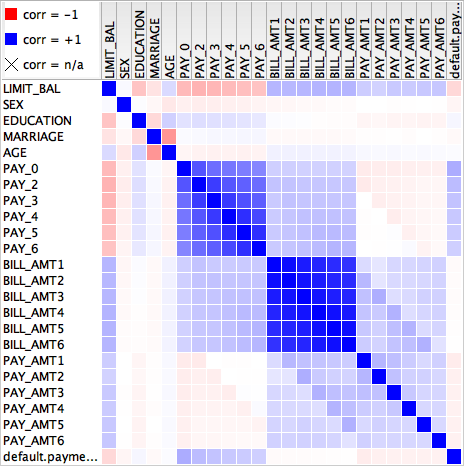
\includegraphics[width=\linewidth]{correlation.png}
		\caption{Correlation Plot of all the attributes}
	\end{figure}
	
	
	The \textit{BILL\_AMT1, $\hdots$,BILL\_AMT6} are heavely correlated; the best option is to create a new feature which is the mean of these colums, called \textit{AVG\_BILL}.
	We decide to compute the average because the bill indicates how much a person spends and it usually remains constant during the months. We remove the \textit{BILL\_AMT1, $\hdots$,BILL\_AMT6} attributes.
	
	For the \textit{AGE} attribute we decide to discretize, creating 4 groups: $\{[20,30],(30,40],(40,50],(50,+\infty)\}$.
	The choice to discretize is made to avoid the possible overfitting phenomena since the \textit{AGE} attribute is imbalanced.
	
	In the \textit{EDUCATION} attribute we combine \textit{0=others} with \textit{3=others} (it is considered to be divorced or separated).
	We combine \textit{SEX} and \textit{MARRIAGE} to reduce the dimension using the following python code:
	
		
\begin{lstlisting}
#df is our dataframe given in the input node
df.loc[((df.SEX == 1) & (df.MARRIAGE == 1)) , 'SEX_MARRIAGE'] = 1 #married man
df.loc[((df.SEX == 1) & (df.MARRIAGE == 2)) , 'SEX_MARRIAGE'] = 2 #single man
df.loc[((df.SEX == 1) & (df.MARRIAGE == 3)) , 'SEX_MARRIAGE'] = 3 #divorced man
df.loc[((df.SEX == 2) & (df.MARRIAGE == 1)) , 'SEX_MARRIAGE'] = 4 #married woman
df.loc[((df.SEX == 2) & (df.MARRIAGE == 2)) , 'SEX_MARRIAGE'] = 5 #single woman
df.loc[((df.SEX == 2) & (df.MARRIAGE == 3)) , 'SEX_MARRIAGE'] = 6 #divorced woman
\end{lstlisting}
	
	Due to the distribution of \textit{LIMIT\_BAL, PAY\_AMT1,$\hdots$, PAY\_AMT6, AVG\_BILL\_AMT} we use the logarithmic transformation. Since there are negative values, we translate the minimum to 1 and apply the logarithm to the later. We notice that the distribution of the \textit{AVG\_BILL\_AMT} has one strong outlier so we remove it to avoid overfitting and standardize the latter for it to be more sparse.
	
	To start studing the classifiers we split our data in training set(67\%) and test set(33\%), using a stratified sampling on \textit{default.payment.next.month}.
	
	\section{Classification}
	The models selected for the classifications are: 
	\begin{itemize}[noitemsep]
		\item MLP
		\item Support Vector Machine: SPegasos
		\item NaiveBayes
		
		\item Bayesian Network:
		\begin{itemize}[noitemsep]
				\item NBTree
				\item BayesNet
		\end{itemize}
		
		\item  Heuristic:
		\begin{itemize}[noitemsep]
			 \item J48
			 \item RandomForest
			 \item DecisionTree
		\end{itemize}
		
		\item Logistic
		
		
	\end{itemize}

	\begin{figure}[h]
	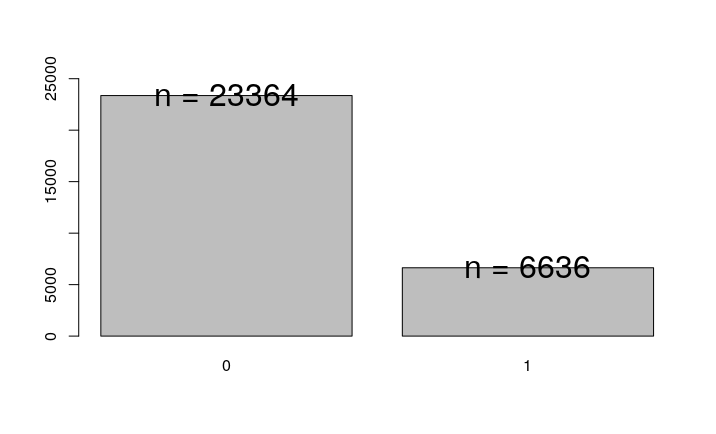
\includegraphics[width=\linewidth]{class.png}
	\caption{Target Class Distribution}
	\end{figure}

The target class has 77.7\% of no defaulters, 22.3\% of defaulters, so we have a class imbalance problem and we cannot use accuracy as an evaluation measure for the classifiers.
The optimal measure could be either Recall or Precision, depending on bank's preference.
We decide to use two measures: harmonic mean between Recall and Precision: $F_1-$measure and AUC of the ROC Curve.

\begin{table}
\resizebox{\columnwidth}{!}{
\begin{tabular}{llllll}
		\toprule
		Classifier & Recall & Precision & $F_1-$measure & Accuracy & AUC\\
		\bottomrule
		\rule{0pt}{3ex}    
		MLP & 0.474 & 0.565 & 0.515 & 0.803 & 0.722\\
		SPegasos & 0.202 & 0.721 & 0.316 & 0.806 & 0.59\\
		NaiveBayes & 0.486 & 0.488 & 0.487 & 0.773 & 0.742\\
		NBTree & 0.481 & 0.53 & 0.504 & 0.791 & 0.754\\
		BayesNet(TANB) & 0.421 & 0.586 & 0.49 & 0.806 & 0.754\\
		J48 & 0.325 & 0.631 & 0.429 & 0.809 & 0.629\\
		RandomForest & 0.325 & 0.612 & 0.425 & 0.805 & 0.723\\
		DecisionTree & 0.401 & 0.402 & 0.401 & 0.736 & 0.635\\
		Logistic & 0.221 & 0.685 & 0.335 & 0.805 & 0.745\\
		\bottomrule
		
\end{tabular}}
\caption{Evaluation measures using holdout}
\end{table}

\noindent

For the Recall Measure NaiveBayes is the optimal classifier, but it has a low precision of 0.488, while using the $F_1-$measure or AUC the best classifiers are MLP, NBTree, BayesNet and NaiveBayes.

%%%%%%%%%%%%%%%%%%%%%%%%%%%%%%%%%%%%%%%%%%
%%Talk about the 3 fold cross validation%%
%%%%%%%%%%%%%%%%%%%%%%%%%%%%%%%%%%%%%%%%%%

\section{Feature Selection}
For the feature selection we use 5 filters:
\begin{itemize}[noitemsep]
	\item Gain Ratio feature evaluation
	\item Information Gain Ranking Filter
	\item Symmetrical Uncertainly Ranking Filter
	\item Relief Ranking Filter(k=10)
	\item Correlation Ranking Filter
\end{itemize}

But all these filters select all attributes. By using these filters we gain no additional information.
The next approach is to use a Wrapper, we decide to use as the classifier BayesNet and NBTree with 10 folds using as evaluation measure AUC.
The wrapper with BayesNet selects 10 attributes:
\begin{itemize}[noitemsep]
\item LIMIT\_BAL
\item EDUCATION
\item PAY\_0
\item PAY\_2
\item PAY\_3
\item PAY\_4
\item PAY\_6
\item PAY\_AMT1
\item PAY\_AMT4
\item SEX\_MARRIAGE
\end{itemize}
While the wrapper with NBTree select the following 10:
\begin{itemize}[noitemsep]
	\item LIMIT\_BAL
	\item EDUCATION
	\item PAY\_0
	\item PAY\_2
	\item PAY\_3
	\item PAY\_6
	\item PAY\_AMT3
	\item PAY\_AMT4
	\item AgeBin
	\item SEX\_MARRIAGE
\end{itemize}

	%----------------------------------------------------------------------------------------
	%	REFERENCE LIST
	%----------------------------------------------------------------------------------------
	\nocite{DataSet}
	\nocite{LucaNoteBook}
	\nocite{Default}
	\nocite{ItalPress}
	\phantomsection
	\bibliographystyle{unsrt}
	\bibliography{biblio}
	
	%----------------------------------------------------------------------------------------
	
\end{document}